% Source Code Guide for Sciara-fv2 CUDA Project
% Chi tiết hướng dẫn cho người mới bắt đầu
\documentclass[11pt,a4paper]{article}

\usepackage[utf8]{inputenc}
\usepackage[margin=2cm]{geometry}
\usepackage{graphicx}
\usepackage{booktabs}
\usepackage{xcolor}
\usepackage{listings}
\usepackage{tikz}
\usetikzlibrary{shapes.geometric, arrows, positioning}
\usepackage{hyperref}
\usepackage{tcolorbox}
\usepackage{enumitem}

% Code listing style
\lstset{
    language=C++,
    basicstyle=\ttfamily\footnotesize,
    keywordstyle=\color{blue}\bfseries,
    commentstyle=\color{green!60!black}\itshape,
    stringstyle=\color{red!70!black},
    numbers=left,
    numberstyle=\tiny\color{gray},
    breaklines=true,
    frame=single,
    backgroundcolor=\color{gray!5},
    tabsize=4,
    morekeywords={__global__, __device__, __shared__, __constant__, dim3, cudaMallocManaged, cudaMemcpy, cudaFree, atomicAdd}
}

% Custom boxes
\newtcolorbox{purposebox}[1][]{colback=blue!5, colframe=blue!75!black, title={\textbf{MỤC ĐÍCH}}, #1}
\newtcolorbox{keypoint}[1][]{colback=yellow!10, colframe=orange!75!black, title={\textbf{ĐIỂM QUAN TRỌNG}}, #1}
\newtcolorbox{newbie}[1][]{colback=green!5, colframe=green!50!black, title={\textbf{GIẢI THÍCH CHO NEWBIE}}, #1}
\newtcolorbox{originbox}[1][]{colback=purple!5, colframe=purple!75!black, title={\textbf{NGUỒN GỐC FILE}}, #1}

\title{\Huge\textbf{Hướng Dẫn Source Code}\\[0.5em]
\Large Sciara-fv2 CUDA Lava Flow Simulator\\[0.5em]
\normalsize Giải thích chi tiết từng đoạn code cho người mới}
\author{Auto-generated Documentation}
\date{\today}

\begin{document}

\maketitle
\tableofcontents
\newpage

%==============================================================================
\section{Tổng Quan Project}
%==============================================================================

\subsection{Project này làm gì?}

\begin{newbie}
Sciara-fv2 mô phỏng dòng chảy của \textbf{dung nham núi lửa} (lava flow).
Tưởng tượng bạn có một lưới ô vuông (như bàn cờ vua), mỗi ô chứa thông tin:
\begin{itemize}
    \item \textbf{Sz}: Độ cao địa hình (altitude) - núi cao, thung lũng thấp
    \item \textbf{Sh}: Độ dày lava (thickness) - bao nhiêu lava đang ở ô này
    \item \textbf{ST}: Nhiệt độ lava (temperature) - nóng thì chảy, nguội thì đông
\end{itemize}
Mỗi bước thời gian, lava chảy từ ô cao xuống ô thấp theo trọng lực.
\end{newbie}

\subsection{Cấu trúc thư mục}

\begin{verbatim}
draft_sciara-fv2/
├── Sciara.h              <- Header chính: định nghĩa struct, constants
├── Sciara.cpp            <- [CPU] Quản lý bộ nhớ CPU (bản gốc)
├── Sciara.cu             <- [GPU] Quản lý bộ nhớ GPU (Unified Memory)
│
├── sciara_fv2.cpp        <- [CPU] Bản serial chạy trên CPU (tham khảo)
├── sciara_fv2.cu         <- [GPU] Version 1: Global Memory (BASELINE)
├── sciara_fv2_tiled.cu   <- [GPU] Version 2: Shared Memory (no halo)
├── sciara_fv2_tiled_halo.cu <- [GPU] Version 3: Shared Memory + Halo
├── sciara_fv2_cfame.cu   <- [GPU] Version 4: Atomic (giữ buffer Mf)
├── sciara_fv2_cfamo.cu   <- [GPU] Version 5: Atomic (bỏ Mf) - NHANH NHẤT
│
├── block_size_exploration.cu <- Tool benchmark kích thước block
├── io.cpp, vent.cpp, ... <- Các file hỗ trợ I/O
└── data/                 <- Dữ liệu Mt. Etna 2006
\end{verbatim}

%==============================================================================
\section{Sơ Đồ Phát Triển Các File CUDA}
%==============================================================================

\begin{center}
\begin{tikzpicture}[
    node distance=1.2cm,
    box/.style={rectangle, draw, rounded corners, minimum width=4cm, minimum height=1cm, align=center, fill=blue!10},
    arrow/.style={->, thick, >=stealth}
]

% Row 1: Original
\node[box, fill=gray!30] (cpp) {Sciara.cpp\\(CPU memory - bản gốc)};
\node[box, fill=gray!30, right=3cm of cpp] (serial) {sciara\_fv2.cpp\\(CPU serial - tham khảo)};

% Row 2: CUDA base
\node[box, fill=yellow!30, below=of cpp] (cu) {Sciara.cu\\(GPU Unified Memory)};
\node[box, fill=green!30, below=of serial] (global) {sciara\_fv2.cu\\(Global Memory - BASELINE)};

% Row 3: Branches
\node[box, fill=cyan!30, below left=1.5cm and -0.5cm of global] (tiled) {sciara\_fv2\_tiled.cu\\(Shared Memory)};
\node[box, fill=orange!30, below right=1.5cm and -0.5cm of global] (cfame) {sciara\_fv2\_cfame.cu\\(Atomic Scatter)};

% Row 4: Final
\node[box, fill=cyan!50, below=of tiled] (halo) {sciara\_fv2\_tiled\_halo.cu\\(+ Halo Region)};
\node[box, fill=red!40, below=of cfame] (cfamo) {sciara\_fv2\_cfamo.cu\\(Bỏ buffer Mf)\\NHANH NHẤT};

% Standalone
\node[box, fill=purple!20, right=2cm of global] (explore) {block\_size\_exploration.cu\\(Benchmark tool)};

% Arrows
\draw[arrow] (cpp) -- (cu) node[midway, left, font=\scriptsize] {malloc→cudaMallocManaged};
\draw[arrow] (serial) -- (global) node[midway, right, font=\scriptsize] {Thêm CUDA kernels};
\draw[arrow] (cu) -- (global) node[midway, above, font=\scriptsize] {dùng chung};
\draw[arrow] (global) -- (tiled) node[midway, left, font=\scriptsize] {+shared mem};
\draw[arrow] (global) -- (cfame) node[midway, right, font=\scriptsize] {merge kernels};
\draw[arrow] (tiled) -- (halo) node[midway, left, font=\scriptsize] {+halo};
\draw[arrow] (cfame) -- (cfamo) node[midway, right, font=\scriptsize] {bỏ Mf};
\draw[arrow, dashed] (global) -- (explore);

\end{tikzpicture}
\end{center}

%==============================================================================
\section{Sciara.h - Header File (Định nghĩa cấu trúc)}
%==============================================================================

\begin{originbox}
\textbf{File gốc}, không thay đổi qua các version. Định nghĩa tất cả struct và constants dùng chung.
\end{originbox}

\subsection{Constants quan trọng}

\begin{lstlisting}[caption={Các hằng số quan trọng trong Sciara.h}]
#define VON_NEUMANN_NEIGHBORS 5   // 4 neighbors + center
#define MOORE_NEIGHBORS 9         // 8 neighbors + center
#define NUMBER_OF_OUTFLOWS 8      // 8 hướng chảy ra

// Moore neighborhood layout:
//    [5] [1] [8]
//    [2] [0] [3]    <- [0] là cell trung tâm
//    [6] [4] [7]
\end{lstlisting}

\begin{newbie}
\textbf{Moore Neighborhood} = 8 ô xung quanh + ô trung tâm = 9 ô.
Lava có thể chảy theo 8 hướng (trái, phải, trên, dưới, 4 góc chéo).
\end{newbie}

\subsection{Struct Substates - Dữ liệu mô phỏng}

\begin{lstlisting}[caption={Struct chứa tất cả mảng dữ liệu}]
typedef struct {
    double* Sz;      // Altitude - độ cao địa hình
    double* Sz_next; // Altitude sau bước tiếp theo
    double* Sh;      // Lava thickness - độ dày lava hiện tại
    double* Sh_next; // Thickness sau bước tiếp theo
    double* ST;      // Temperature - nhiệt độ lava
    double* ST_next; // Temperature sau bước tiếp theo
    double* Mf;      // Flow matrix - lưu lượng chảy (8 hướng x cells)
    bool*   Mb;      // Boundary mask - đánh dấu ô biên
    double* Mhs;     // Solidified height - lava đã đông đặc
} Substates;
\end{lstlisting}

\begin{keypoint}
Tại sao có \texttt{\_next}? Đây là kỹ thuật \textbf{Double Buffering}:
\begin{itemize}
    \item Đọc từ \texttt{Sh} (giá trị hiện tại)
    \item Ghi vào \texttt{Sh\_next} (giá trị mới)
    \item Cuối bước: swap \texttt{Sh} và \texttt{Sh\_next}
\end{itemize}
Tránh race condition khi nhiều thread đọc/ghi cùng lúc.
\end{keypoint}

%==============================================================================
\section{Sciara.cpp vs Sciara.cu - Quản lý bộ nhớ}
%==============================================================================

\begin{originbox}
\textbf{Sciara.cpp} = bản CPU gốc, dùng \texttt{new/delete}\\
\textbf{Sciara.cu} = bản GPU, dùng \texttt{cudaMallocManaged/cudaFree}
\end{originbox}

\subsection{So sánh cấp phát bộ nhớ}

\begin{lstlisting}[caption={CPU (Sciara.cpp) vs GPU (Sciara.cu)}]
// ===== Sciara.cpp (CPU) =====
void allocateSubstates(Sciara *sciara) {
    int size = rows * cols;
    sciara->substates->Sz = new double[size]();  // CPU heap
    // ... tương tự cho các mảng khác
}

// ===== Sciara.cu (GPU) =====
void allocateSubstates(Sciara *sciara) {
    int size = rows * cols;
    // Unified Memory: CPU và GPU đều truy cập được!
    cudaMallocManaged(&sciara->substates->Sz, sizeof(double) * size);
    // ... tương tự cho các mảng khác
}
\end{lstlisting}

\begin{newbie}
\textbf{cudaMallocManaged} là gì?
\begin{itemize}
    \item \texttt{malloc/new}: Chỉ CPU đọc/ghi được
    \item \texttt{cudaMalloc}: Chỉ GPU đọc/ghi được
    \item \texttt{cudaMallocManaged}: \textbf{CẢ HAI} CPU và GPU đều đọc/ghi được!
\end{itemize}
Driver CUDA tự động copy dữ liệu khi cần. Rất tiện nhưng có overhead.
\end{newbie}

%==============================================================================
\section{sciara\_fv2.cu - Global Memory Version (BASELINE)}
%==============================================================================

\begin{originbox}
\textbf{Phát triển từ}: sciara\_fv2.cpp (CPU serial)\\
\textbf{Thay đổi}: Chuyển các hàm thành CUDA kernels, thêm parallel execution
\end{originbox}

\begin{purposebox}
Version cơ bản nhất. Tất cả kernel đọc/ghi trực tiếp từ \textbf{Global Memory}.
Dùng làm baseline để so sánh với các version tối ưu.
\end{purposebox}

\subsection{Cấu hình CUDA}

\begin{lstlisting}[caption={Cấu hình block và grid}]
#define BLOCK_SIZE_X 16
#define BLOCK_SIZE_Y 16

// Trong main():
dim3 blockDim(BLOCK_SIZE_X, BLOCK_SIZE_Y);  // 16x16 = 256 threads/block
dim3 gridDim((cols + 15) / 16, (rows + 15) / 16);  // 33x24 blocks
// Tổng: 33*24 = 792 blocks, 792*256 = 202,752 threads
\end{lstlisting}

\begin{newbie}
\textbf{Thread hierarchy trong CUDA}:
\begin{verbatim}
Grid (toàn bộ)
├── Block (0,0): 256 threads
├── Block (0,1): 256 threads
├── ...
└── Block (32,23): 256 threads

Mỗi thread xử lý 1 cell trong grid 517x378
\end{verbatim}
\end{newbie}

\subsection{Macro truy cập mảng 2D}

\begin{lstlisting}[caption={Macro GET/SET cho mảng 2D linearized}]
// Mảng 2D được lưu như mảng 1D: M[i][j] -> M[i*cols + j]
#define GET(M, cols, i, j) (M[((i) * (cols)) + (j)])
#define SET(M, cols, i, j, val) ((M)[((i) * (cols)) + (j)] = (val))

// Mảng 3D cho flows: Mf[direction][i][j]
#define BUF_GET(M, rows, cols, n, i, j) M[((n)*(rows)*(cols)) + ((i)*(cols)) + (j)]
#define BUF_SET(M, rows, cols, n, i, j, val) ...
\end{lstlisting}

\subsection{Constant Memory cho neighbor offsets}

\begin{lstlisting}[caption={Dùng constant memory cho dữ liệu read-only}]
// Host arrays
int h_Xi[] = {0, -1,  0,  0,  1, -1,  1,  1, -1};
int h_Xj[] = {0,  0, -1,  1,  0, -1, -1,  1,  1};

// Device constant memory (nhanh, cached)
__constant__ int d_Xi[MOORE_NEIGHBORS];
__constant__ int d_Xj[MOORE_NEIGHBORS];

// Copy 1 lần khi khởi tạo:
cudaMemcpyToSymbol(d_Xi, h_Xi, MOORE_NEIGHBORS * sizeof(int));
\end{lstlisting}

\begin{keypoint}
\textbf{Constant Memory} nhanh hơn Global Memory vì:
\begin{itemize}
    \item Được cache trên mỗi SM
    \item Broadcast đến tất cả threads trong warp
    \item Chỉ dùng cho dữ liệu read-only, nhỏ ($<$64KB)
\end{itemize}
\end{keypoint}

\subsection{kernel\_emitLava - Phun lava từ miệng núi lửa}

\begin{lstlisting}[caption={Kernel đơn giản nhất - thêm lava vào ô vent}]
__global__ void kernel_emitLava(
    int r, int c,
    int* vent_x, int* vent_y, double* vent_thickness,
    int num_vents, double PTvent,
    double* Sh, double* Sh_next, double* ST_next)
{
    // Tính vị trí cell từ thread ID
    int j = blockIdx.x * blockDim.x + threadIdx.x;
    int i = blockIdx.y * blockDim.y + threadIdx.y;

    if (i >= r || j >= c) return;  // Bounds check

    // Kiểm tra cell này có phải là vent không
    for (int k = 0; k < num_vents; k++) {
        if (i == vent_y[k] && j == vent_x[k]) {
            // Thêm lava vào ô này
            double current_h = GET(Sh, c, i, j);
            SET(Sh_next, c, i, j, current_h + vent_thickness[k]);
            SET(ST_next, c, i, j, PTvent);  // Nhiệt độ vent
        }
    }
}
\end{lstlisting}

\subsection{kernel\_computeOutflows - Kernel NẶNG NHẤT}

\begin{lstlisting}[caption={Tính lượng lava chảy ra mỗi hướng (350 FLOPs/cell)}]
__global__ void kernel_computeOutflows(
    int r, int c,
    double* Sz, double* Sh, double* ST, double* Mf,
    double Pc, double _a, double _b, double _c, double _d)
{
    int j = blockIdx.x * blockDim.x + threadIdx.x;
    int i = blockIdx.y * blockDim.y + threadIdx.y;
    if (i >= r || j >= c) return;

    double h0 = GET(Sh, c, i, j);
    if (h0 <= 0) return;  // Không có lava -> skip

    // Tính viscosity từ temperature (power law)
    double T = GET(ST, c, i, j);
    double rr = pow(10.0, _a + _b * T);  // resistance
    double hc = pow(10.0, _c + _d * T);  // critical height

    // ===== MINIMIZATION ALGORITHM =====
    // Tìm các neighbor mà lava có thể chảy đến
    for (int k = 0; k < MOORE_NEIGHBORS; k++) {
        int ni = i + d_Xi[k];  // Neighbor row
        int nj = j + d_Xj[k];  // Neighbor col

        // ... tính gradient, loại bỏ uphill neighbors ...
    }

    // Tính average height và flow distribution
    // ... (phức tạp, ~100 dòng code) ...

    // Lưu flow vào buffer Mf
    for (int k = 1; k < MOORE_NEIGHBORS; k++) {
        BUF_SET(Mf, r, c, k-1, i, j, flow[k]);
    }
}
\end{lstlisting}

\begin{newbie}
\textbf{Minimization Algorithm} làm gì?
\begin{enumerate}
    \item Nhìn 8 ô xung quanh
    \item Loại bỏ ô cao hơn ô hiện tại (lava không chảy ngược lên)
    \item Tính trung bình độ cao các ô còn lại
    \item Phân phối lava sao cho tất cả ô có cùng độ cao
\end{enumerate}
\end{newbie}

\subsection{kernel\_massBalance - Cập nhật sau khi chảy}

\begin{lstlisting}[caption={Gather inflows từ neighbors}]
__global__ void kernel_massBalance(
    int r, int c,
    double* Sh, double* ST, double* Mf,
    double* Sh_next, double* ST_next)
{
    int j = blockIdx.x * blockDim.x + threadIdx.x;
    int i = blockIdx.y * blockDim.y + threadIdx.y;
    if (i >= r || j >= c) return;

    double h_new = GET(Sh, c, i, j);
    double T_sum = h_new * GET(ST, c, i, j);

    // Trừ lava chảy ĐI từ cell này
    for (int k = 1; k < MOORE_NEIGHBORS; k++) {
        double outflow = BUF_GET(Mf, r, c, k-1, i, j);
        h_new -= outflow;
    }

    // Cộng lava chảy VÀO từ neighbors
    for (int k = 1; k < MOORE_NEIGHBORS; k++) {
        int ni = i + d_Xi[k];
        int nj = j + d_Xj[k];
        if (ni >= 0 && ni < r && nj >= 0 && nj < c) {
            int opposite = ...;  // Hướng ngược lại
            double inflow = BUF_GET(Mf, r, c, opposite, ni, nj);
            h_new += inflow;
            T_sum += inflow * GET(ST, c, ni, nj);
        }
    }

    SET(Sh_next, c, i, j, h_new);
    SET(ST_next, c, i, j, h_new > 0 ? T_sum / h_new : 0);
}
\end{lstlisting}

%==============================================================================
\section{sciara\_fv2\_tiled.cu - Shared Memory (Không Halo)}
%==============================================================================

\begin{originbox}
\textbf{Phát triển từ}: sciara\_fv2.cu (Global Memory)\\
\textbf{Thay đổi}: Thêm shared memory cho các kernel stencil
\end{originbox}

\begin{purposebox}
Tối ưu bằng cách load dữ liệu vào \textbf{Shared Memory} (bộ nhớ nhanh trên chip).
Mỗi block load 1 tile (16x16) vào shared memory trước khi tính toán.
\end{purposebox}

\subsection{Khai báo Shared Memory}

\begin{lstlisting}[caption={Shared memory cho 1 tile}]
#define TILE_SIZE_X 16
#define TILE_SIZE_Y 16

__global__ void kernel_computeOutflows_tiled(...) {
    // Shared memory - chung cho cả block
    __shared__ double s_Sz[TILE_SIZE_Y][TILE_SIZE_X];  // 16x16 doubles
    __shared__ double s_Sh[TILE_SIZE_Y][TILE_SIZE_X];  // = 2KB
    __shared__ double s_ST[TILE_SIZE_Y][TILE_SIZE_X];  // Tổng: 6KB

    int tx = threadIdx.x;  // Local thread x trong block
    int ty = threadIdx.y;  // Local thread y trong block

    // Mỗi thread load 1 element
    if (i < r && j < c) {
        s_Sz[ty][tx] = GET(Sz, c, i, j);
        s_Sh[ty][tx] = GET(Sh, c, i, j);
        s_ST[ty][tx] = GET(ST, c, i, j);
    }
    __syncthreads();  // Đợi TẤT CẢ threads load xong!

    // Giờ dùng s_Sz, s_Sh, s_ST thay vì đọc global
}
\end{lstlisting}

\begin{newbie}
\textbf{Shared Memory} là gì?
\begin{itemize}
    \item Bộ nhớ nhỏ (48KB/SM) nhưng CỰC NHANH (100x so với global)
    \item Dùng chung cho tất cả threads trong 1 block
    \item Phải dùng \texttt{\_\_syncthreads()} để đồng bộ
\end{itemize}
\end{newbie}

\subsection{Vấn đề: Threads ở biên tile}

\begin{lstlisting}[caption={Threads ở biên phải đọc global memory}]
// Thread ở vị trí (0, 0) trong tile cần đọc neighbor (-1, -1)
// Nhưng (-1, -1) nằm NGOÀI tile -> không có trong shared memory!

if (tx == 0 && ty == 0) {
    // Phải đọc từ global memory (CHẬM!)
    neighbor_val = GET(Sz, c, i-1, j-1);
} else {
    // Đọc từ shared memory (NHANH!)
    neighbor_val = s_Sz[ty-1][tx-1];
}
\end{lstlisting}

\begin{keypoint}
Khoảng 25\% threads (ở biên tile) vẫn phải đọc global memory.\\
$\Rightarrow$ Cần \textbf{Halo version} để giải quyết!
\end{keypoint}

%==============================================================================
\section{sciara\_fv2\_tiled\_halo.cu - Shared Memory + Halo}
%==============================================================================

\begin{originbox}
\textbf{Phát triển từ}: sciara\_fv2\_tiled.cu\\
\textbf{Thay đổi}: Load thêm 1 lớp halo xung quanh tile
\end{originbox}

\begin{purposebox}
Giải quyết vấn đề border bằng cách load thêm 1 lớp ô bao quanh tile (\textbf{halo}).
Tile 16x16 trở thành 18x18 trong shared memory.
\end{purposebox}

\subsection{Visualize Halo Region}

\begin{center}
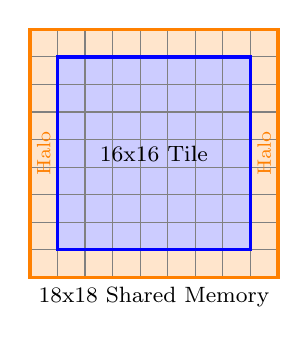
\begin{tikzpicture}[scale=0.35]
% Halo (outer)
\fill[orange!20] (0,0) rectangle (9,9);
% Tile (inner)
\fill[blue!20] (1,1) rectangle (8,8);

\draw[step=1, gray] (0,0) grid (9,9);
\draw[blue, very thick] (1,1) rectangle (8,8);
\draw[orange, very thick] (0,0) rectangle (9,9);

\node at (4.5, 4.5) {\footnotesize 16x16 Tile};
\node[orange] at (0.5, 4.5) {\rotatebox{90}{\scriptsize Halo}};
\node[orange] at (8.5, 4.5) {\rotatebox{90}{\scriptsize Halo}};
\node at (4.5, -0.7) {\footnotesize 18x18 Shared Memory};
\end{tikzpicture}
\end{center}

\begin{lstlisting}[caption={Shared memory với halo}]
#define TILE_SIZE 16
#define HALO 1
#define BLOCK_DIM (TILE_SIZE + 2*HALO)  // 18

__shared__ double s_Sz[BLOCK_DIM][BLOCK_DIM];  // 18x18 = 2.6KB
__shared__ double s_Sh[BLOCK_DIM][BLOCK_DIM];
__shared__ double s_ST[BLOCK_DIM][BLOCK_DIM];  // Tổng: 7.8KB
\end{lstlisting}

\subsection{Load Halo phức tạp hơn}

\begin{lstlisting}[caption={Load tile 16x16 + halo vào shared memory 18x18}]
// 256 threads load 324 elements (18x18)
// Mỗi thread có thể phải load 2 elements

int tx = threadIdx.x + 1;  // +1 vì halo
int ty = threadIdx.y + 1;

// Load center tile (tất cả threads)
s_Sz[ty][tx] = GET(Sz, c, i, j);

// Load halo (chỉ một số threads)
if (threadIdx.x == 0 && j > 0)
    s_Sz[ty][0] = GET(Sz, c, i, j-1);      // Left halo
if (threadIdx.x == 15 && j < c-1)
    s_Sz[ty][17] = GET(Sz, c, i, j+1);     // Right halo
// ... tương tự cho top, bottom, corners

__syncthreads();  // QUAN TRỌNG!
\end{lstlisting}

\begin{keypoint}
\textbf{Tại sao Tiled versions chậm hơn Global trên grid nhỏ?}
\begin{enumerate}
    \item \texttt{\_\_syncthreads()} tốn ~50 cycles mỗi lần
    \item L2 Cache của GTX 980 (2MB) đã đủ lớn cache toàn bộ data
    \item Overhead load halo không bù đắp được lợi ích
\end{enumerate}
Tiled chỉ tốt khi grid $>$ 2048x2048 (vượt L2 cache).
\end{keypoint}

%==============================================================================
\section{sciara\_fv2\_cfame.cu - Atomic Scatter Pattern}
%==============================================================================

\begin{originbox}
\textbf{Phát triển từ}: sciara\_fv2.cu (Global Memory)\\
\textbf{Thay đổi}: Thay đổi từ Gather sang Scatter, gộp 2 kernels
\end{originbox}

\begin{purposebox}
Thay đổi từ \textbf{Gather} (đọc từ neighbors) sang \textbf{Scatter} (ghi đến neighbors).
Gộp \texttt{computeOutflows} và \texttt{massBalance} thành 1 kernel, dùng \textbf{atomic operations}.
\end{purposebox}

\subsection{Gather vs Scatter Pattern}

\begin{center}
\begin{tikzpicture}[scale=0.7]
% Gather
\begin{scope}
\node at (2, 3.5) {\textbf{Gather (Truyền thống)}};
\fill[blue!30] (2,1.5) circle (0.4);
\node at (2, 1.5) {\tiny 0};
\foreach \x/\y/\n in {1/2.2/5, 2/2.6/1, 3/2.2/8, 0.8/1.5/2, 3.2/1.5/3, 1/0.8/6, 2/0.4/4, 3/0.8/7} {
    \fill[gray!30] (\x, \y) circle (0.25);
    \draw[->, thick] (\x, \y) -- (2, 1.5);
}
\node at (2, -0.5) {\scriptsize Cell ĐỌC từ neighbors};
\end{scope}

% Scatter
\begin{scope}[xshift=7cm]
\node at (2, 3.5) {\textbf{Scatter (CfA)}};
\fill[blue!30] (2,1.5) circle (0.4);
\node at (2, 1.5) {\tiny 0};
\foreach \x/\y in {1/2.2, 2/2.6, 3/2.2, 0.8/1.5, 3.2/1.5, 1/0.8, 2/0.4, 3/0.8} {
    \fill[gray!30] (\x, \y) circle (0.25);
    \draw[->, thick, red] (2, 1.5) -- (\x, \y);
}
\node at (2, -0.5) {\scriptsize Cell GHI đến neighbors};
\end{scope}
\end{tikzpicture}
\end{center}

\subsection{Tại sao cần Atomic Operations?}

\begin{lstlisting}[caption={Race condition khi nhiều threads ghi cùng ô}]
// KHÔNG có atomic - SAI!
// Thread A (cell 1): Sh_next[X] = Sh_next[X] + flow_A
// Thread B (cell 2): Sh_next[X] = Sh_next[X] + flow_B
// Nếu chạy song song: chỉ 1 giá trị được lưu, mất dữ liệu!

// CÓ atomic - ĐÚNG!
atomicAddDouble(&Sh_next[X], flow_A);  // Thread A
atomicAddDouble(&Sh_next[X], flow_B);  // Thread B
// Cả 2 giá trị đều được cộng đúng
\end{lstlisting}

\subsection{atomicAddDouble cho FP64}

\begin{lstlisting}[caption={Implement atomic add cho double (FP64)}]
// GTX 980 không có native atomicAdd cho double
// Phải tự implement bằng atomicCAS

__device__ double atomicAddDouble(double* address, double val) {
    unsigned long long int* addr_as_ull = (unsigned long long int*)address;
    unsigned long long int old = *addr_as_ull, assumed;
    do {
        assumed = old;
        old = atomicCAS(addr_as_ull, assumed,
                __double_as_longlong(val + __longlong_as_double(assumed)));
    } while (assumed != old);
    return __longlong_as_double(old);
}
\end{lstlisting}

\subsection{Temperature Accumulation Trick}

\begin{lstlisting}[caption={Trick tính nhiệt độ trung bình với atomic}]
// Vấn đề: Không thể atomic tính trung bình!
// T_avg = (h1*T1 + h2*T2 + ...) / (h1 + h2 + ...)

// Giải pháp: Lưu h*T thay vì T
kernel_initBuffers<<<...>>>() {
    ST_next[i] = Sh[i] * ST[i];  // Lưu TÍCH h*T
}

kernel_CfA_Me<<<...>>>() {
    atomicAddDouble(&Sh_next[neighbor], flow);
    atomicAddDouble(&ST_next[neighbor], flow * T);  // Cộng thêm flow*T
}

kernel_normalizeTemperature<<<...>>>() {
    if (Sh_next[i] > 0)
        ST_next[i] = ST_next[i] / Sh_next[i];  // T = (h*T) / h
}
\end{lstlisting}

%==============================================================================
\section{sciara\_fv2\_cfamo.cu - Memory Optimized (NHANH NHẤT)}
%==============================================================================

\begin{originbox}
\textbf{Phát triển từ}: sciara\_fv2\_cfame.cu\\
\textbf{Thay đổi}: Bỏ hoàn toàn buffer Mf, tiết kiệm 12.5MB
\end{originbox}

\begin{purposebox}
Tối ưu thêm từ CfAMe bằng cách \textbf{bỏ mảng Mf} (12.5MB).
Flow được tính và áp dụng ngay, không lưu trung gian.
\end{purposebox}

\subsection{So sánh CfAMe vs CfAMo}

\begin{table}[h]
\centering
\begin{tabular}{@{}lcc@{}}
\toprule
& \textbf{CfAMe} & \textbf{CfAMo} \\
\midrule
Buffer Mf & Có (8 × 195,426 × 8 = 12.5 MB) & \textbf{Không} \\
Có thể debug flows & Có & Không \\
Memory bandwidth & Cao hơn & Thấp hơn \\
Số kernel launches & 4 & 3 \\
Speedup vs Global & 0.88× & \textbf{1.09×} \\
\bottomrule
\end{tabular}
\end{table}

\begin{lstlisting}[caption={CfAMo bỏ việc lưu Mf}]
// CfAMe: Lưu flow rồi mới dùng
BUF_SET(Mf, r, c, k-1, i, j, flow);  // Lưu vào Mf
atomicAddDouble(&Sh_next[...], flow);

// CfAMo: Dùng flow trực tiếp, KHÔNG lưu
if (flow > 0) {
    atomicAddDouble(&Sh_next[ni * c + nj], flow);
    atomicAddDouble(&ST_next[ni * c + nj], flow * T);
    // KHÔNG có BUF_SET -> tiết kiệm memory
}
\end{lstlisting}

\begin{keypoint}
\textbf{Tại sao CfAMo nhanh nhất?}
\begin{enumerate}
    \item \textbf{Ít memory}: Không có Mf 12.5MB $\Rightarrow$ cache hit tốt hơn
    \item \textbf{Ít kernel launches}: 3 thay vì 4 (tiết kiệm overhead)
    \item \textbf{Atomic contention thấp}: Chỉ ~5\% cells có lava active
\end{enumerate}
\end{keypoint}

%==============================================================================
\section{block\_size\_exploration.cu - Tool Benchmark}
%==============================================================================

\begin{originbox}
\textbf{File độc lập}, không phụ thuộc vào các file khác.\\
Mục đích: Test các kích thước block để tìm cấu hình tối ưu.
\end{originbox}

\begin{lstlisting}[caption={Chạy benchmark tool}]
$ nvcc -O3 -arch=sm_52 block_size_exploration.cu -o block_explore
$ ./block_explore

| Block | Thrds | Grid Size | Neighbor | Elemwise | Occupancy |
|-------|-------|-----------|----------|----------|-----------|
| 8x8   |  64   | (65, 48)  |   0.125  |   0.042  |   50.0%   |
|16x16  | 256   | (33, 24)  |   0.098  |   0.038  |  100.0%   | <- TỐT
|32x32  |1024   | (17, 12)  |   0.112  |   0.041  |   50.0%   |
\end{lstlisting}

%==============================================================================
\section{Tổng Kết}
%==============================================================================

\begin{table}[h]
\centering
\caption{So sánh 5 CUDA versions}
\begin{tabular}{@{}lcccl@{}}
\toprule
\textbf{File} & \textbf{Technique} & \textbf{Time} & \textbf{Speedup} & \textbf{Khi nào dùng?} \\
\midrule
sciara\_fv2.cu & Global Memory & 21.6s & 1.00× & Debug, verify \\
sciara\_fv2\_tiled.cu & Shared mem & 20.1s & 1.07× & Grid > 2048×2048 \\
sciara\_fv2\_tiled\_halo.cu & +Halo & 23.3s & 0.93× & Grid > 2048×2048 \\
sciara\_fv2\_cfame.cu & Atomic scatter & 24.7s & 0.88× & Cần debug flow \\
\textbf{sciara\_fv2\_cfamo.cu} & \textbf{+Bỏ Mf} & \textbf{19.7s} & \textbf{1.09×} & \textbf{Production} \\
\bottomrule
\end{tabular}
\end{table}

\begin{newbie}
\textbf{Kết luận cho người mới:}
\begin{itemize}
    \item Với grid nhỏ ($<$ 2048×2048), dùng \textbf{CfAMo} (nhanh nhất)
    \item Shared memory tiling chỉ tốt khi grid lớn hơn L2 cache
    \item High occupancy $\neq$ Fast (CfAMo occupancy thấp nhưng nhanh nhất)
    \item Bộ nhớ ít hơn = cache hit tốt hơn = nhanh hơn
\end{itemize}
\end{newbie}

\end{document}
